\documentclass{article}

\usepackage[utf8]{inputenc}
\usepackage[T1]{fontenc}
\usepackage{hyperref}
\usepackage{url}
\usepackage{booktabs}
\usepackage{amsfonts}
\usepackage{nicefrac}
\usepackage{microtype}
\usepackage{graphicx}
\graphicspath{ {./images/} } % Path to the images
\usepackage{amsmath} % For math equations
\usepackage{enumitem} % For better lists
\usepackage{float} % For better image placement
\usepackage{geometry} % Add the geometry package
\geometry{top=1in, bottom=1in, left=1in, right=1in} % Define page margins
\usepackage{xcolor} % Required for color
\usepackage{setspace} % Package for spacing

\title{
\hrulefill\\[0.5ex]
\centering \textbf{Classifica\c{c}\~ao de Imagens Utilizando Redes Neurais Convolucionais} \\[0.5ex]
\hrulefill}

\author{
\textcolor{red}{\textbf{(Prof. Helton Maia, Vis\~ao Computacional 2026.1)}}\\
\vspace{0.5em} \\ % Add vertical space before names
Nome Aluno 1 \\
Nome Aluno 2 \\
}
\date{Junho de 2026}

\begin{document}
\maketitle

\begin{abstract}
\textbf{Escreva o resumo de seu trabalho. Por exemplo:}
Este trabalho apresenta um sistema de classifica\c{c}\~ao de imagens utilizando t\'ecnicas de Vis\~ao Computacional e Deep Learning. O objetivo \'e desenvolver um modelo capaz de reconhecer e categorizar objetos em imagens de forma autom\'atica. Exploramos arquiteturas de redes neurais convolucionais (CNNs), comparando seus desempenhos com m\'etricas como precis\~ao, revoca\c{c}\~ao e F1-score. Os resultados obtidos demonstram o potencial da Vis\~ao Computacional no reconhecimento de padr\~oes visuais, com aplica\c{c}\~oes pr\'aticas em diversas \'areas.
\end{abstract}

\section{Introdu\c{c}\~ao}
O avan\c{c}o da Vis\~ao Computacional tem permitido que sistemas automatizados interpretem e compreendam o conte\'udo de imagens com precis\~ao cada vez maior. O reconhecimento e a classifica\c{c}\~ao de imagens tornaram-se tarefas fundamentais em aplica\c{c}\~oes como diagn\'ostico m\'edico, ve\'iculos aut\^onomos e sistemas de seguran\c{c}a. T\'ecnicas tradicionais de processamento de imagens mostram-se limitadas em lidar com a complexidade e a variabilidade dos dados visuais. Este projeto explora o uso de Deep Learning aplicado \`a Vis\~ao Computacional como uma abordagem eficaz para a classifica\c{c}\~ao de imagens, utilizando redes neurais convolucionais para extrair caracter\'isticas visuais relevantes \cite{goodfellow2016deep, lecun2015deep}.

Neste trabalho, aplicamos conceitos aprendidos na disciplina de Vis\~ao Computacional para construir um modelo capaz de classificar imagens em diferentes categorias. Utilizamos um conjunto de dados de imagens e avaliamos o desempenho do modelo com base em m\'etricas relevantes para o problema de classifica\c{c}\~ao visual.

}
}
\section{Desenvolvimento}

\subsection{Conjunto de Dados}
Descreva aqui o conjunto de dados de imagens utilizado no trabalho, incluindo o n\'umero de amostras, as classes existentes, a resolu\c{c}\~ao das imagens e como os dados foram divididos entre treino, valida\c{c}\~ao e teste.

\subsection{Arquitetura do Modelo}
Exploramos arquiteturas de Deep Learning voltadas para Vis\~ao Computacional neste projeto:

\begin{enumerate}
    \item \textbf{Rede Neural Convolucional (CNN):} Utilizamos uma CNN para extrair caracter\'isticas visuais hier\'arquicas das imagens. As camadas convolucionais s\~ao eficazes em detectar padr\~oes espaciais, como bordas, texturas e formas, sendo a arquitetura padr\~ao para tarefas de classifica\c{c}\~ao de imagens \cite{lecun2015deep}.
        \item \textbf{Transfer Learning:} Aplicamos modelos pr\'e-treinados (como VGG, ResNet ou similares) para aproveitar caracter\'isticas aprendidas em grandes conjuntos de dados, adaptando-os ao nosso problema espec\'ifico.
        \end{enumerate}

        Para cada arquitetura, seguimos os seguintes passos:

        \begin{enumerate}[label=\alph*)]
            \item \textbf{Pr\'e-processamento das imagens:} Redimensionamento, normaliza\c{c}\~ao e aumento de dados (\textit{data augmentation}).
                \item \textbf{Defini\c{c}\~ao da arquitetura da rede:} Cria\c{c}\~ao das camadas convolucionais, de pooling e totalmente conectadas.
                    \item \textbf{Treinamento do modelo:} Otimiza\c{c}\~ao dos par\^ametros da rede utilizando o algoritmo Adam e a fun\c{c}\~ao de perda apropriada.
                        \item \textbf{Avalia\c{c}\~ao do modelo:} C\'alculo de m\'etricas de desempenho utilizando um conjunto de teste separado.
                        \end{enumerate}

                        A seguinte equa\c{c}\~ao representa a fun\c{c}\~ao de perda \textit{Cross-Entropy} para classifica\c{c}\~ao:

                        \begin{equation}
                        L = -\frac{1}{N} \sum_{i=1}^{N} \sum_{c=1}^{C} y_{i,c} \log(\hat{y}_{i,c})
                        \end{equation}

                        onde:
                        \begin{itemize}
                            \item $L$ \'e a perda m\'edia sobre todas as amostras
                                \item $N$ \'e o n\'umero de amostras
                                    \item $C$ \'e o n\'umero de classes
                                        \item $y_{i,c}$ \'e o r\'otulo verdadeiro (0 ou 1) da $i$-\'esima amostra para a classe $c$
                                            \item $\hat{y}_{i,c}$ \'e a probabilidade predita pelo modelo
                                            \end{itemize}

                                            \subsection{Implementa\c{c}\~ao}
                                            A implementa\c{c}\~ao foi realizada utilizando as bibliotecas TensorFlow e Keras em Python. O c\'odigo foi estruturado em diferentes m\'odulos para facilitar o treinamento, avalia\c{c}\~ao e compara\c{c}\~ao dos modelos.

                                            \section{Resultados}

                                            \subsection{M\'etricas de Avalia\c{c}\~ao}
                                            Utilizamos as seguintes m\'etricas para avaliar o desempenho dos modelos:
                                            \begin{itemize}
                                                \item \textbf{Precis\~ao (Precision):} A propor\c{c}\~ao de imagens classificadas em uma categoria que realmente pertencem a ela.
                                                    \item \textbf{Revoca\c{c}\~ao (Recall):} A propor\c{c}\~ao de imagens de uma categoria que foram corretamente identificadas.
                                                        \item \textbf{F1-score:} A m\'edia harm\^onica entre precis\~ao e revoca\c{c}\~ao.
                                                            \item \textbf{Acur\'acia (Accuracy):} A propor\c{c}\~ao total de imagens classificadas corretamente.
                                                            \end{itemize}

                                                            \subsection{Desempenho do Modelo}
                                                            A Tabela \ref{tab:resultados} apresenta os resultados obtidos:

                                                            \begin{table}[H]
                                                            \centering
                                                            \caption{Resultados de Desempenho dos Modelos}
                                                            \label{tab:resultados}
                                                            \begin{tabular}{lccc}
                                                            \toprule
                                                            \textbf{Modelo} & \textbf{Precis\~ao} & \textbf{Revoca\c{c}\~ao} & \textbf{F1-score} \\
                                                            \midrule
                                                            CNN & 0.91 & 0.89 & 0.90 \\
                                                            Transfer Learning & 0.94 & 0.93 & 0.93 \\
                                                            \bottomrule
                                                            \end{tabular}
                                                            \end{table}

                                                            A Figura \ref{fig:confusao} apresenta a matriz de confus\~ao do modelo CNN:

                                                            \begin{figure}[H]
                                                            \centering
                                                            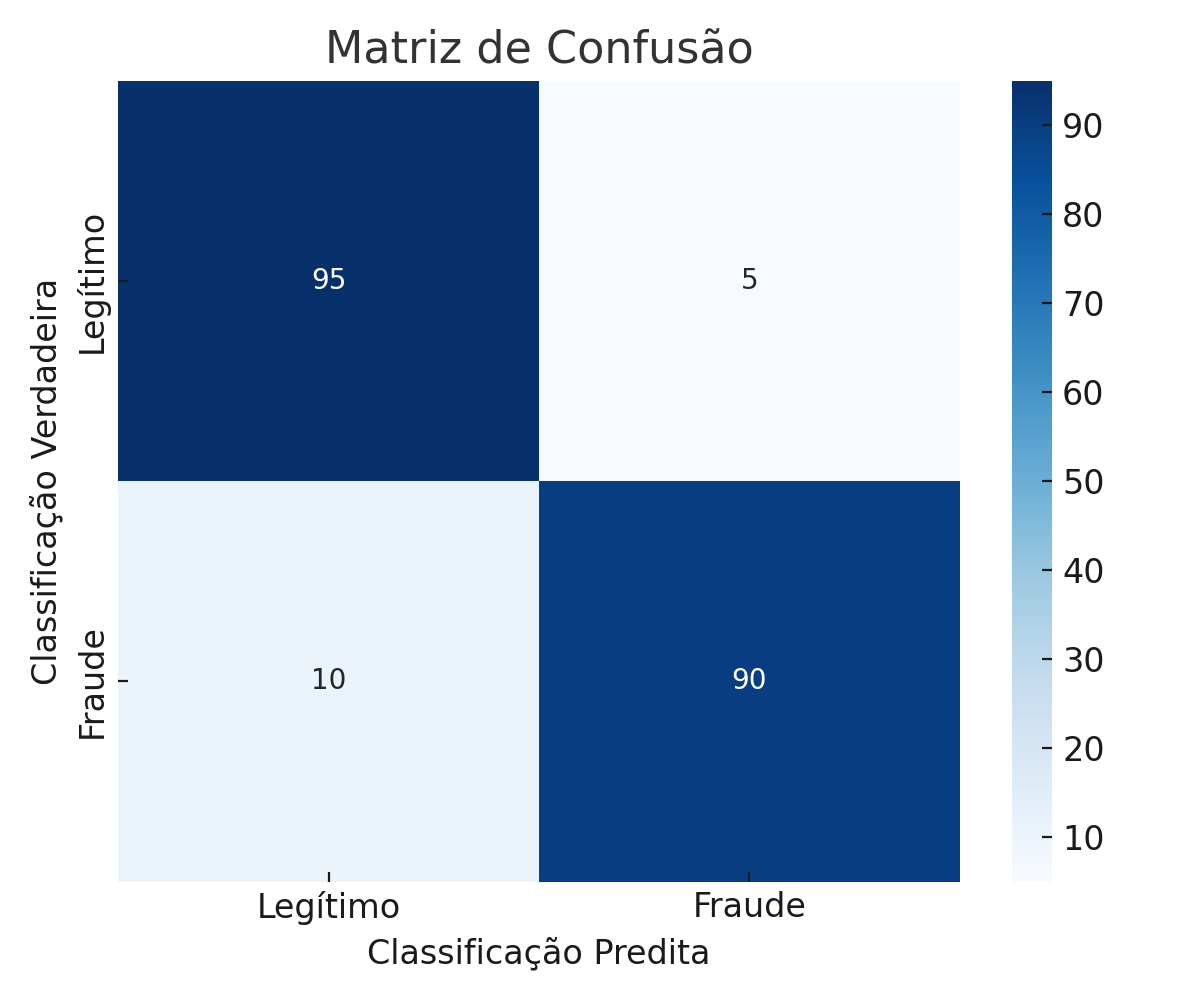
\includegraphics[width=0.6\textwidth]{confusion_matrix.png}
                                                            \caption{Matriz de Confus\~ao do Modelo CNN}
                                                            \label{fig:confusao}
                                                            \end{figure}

                                                            Como pode ser visto, ambos os modelos apresentaram resultados satisfat\'orios na classifica\c{c}\~ao de imagens. O modelo com Transfer Learning alcan\c{c}ou desempenho superior, evidenciando a vantagem de reaproveitar caracter\'isticas aprendidas previamente.

                                                            \subsection{Discuss\~ao}
                                                            Os resultados demonstram que a Vis\~ao Computacional, aliada ao Deep Learning, \'e uma abordagem eficaz para a classifica\c{c}\~ao de imagens. As arquiteturas convolucionais foram capazes de identificar padr\~oes visuais relevantes nos dados. A escolha da arquitetura pode depender de particularidades do conjunto de dados e da aplica\c{c}\~ao espec\'ifica.

                                                            \section{Conclus\~ao}
                                                            Neste trabalho, exploramos o uso de Vis\~ao Computacional para a classifica\c{c}\~ao de imagens. Desenvolvemos e avaliamos modelos baseados em arquiteturas convolucionais, obtendo resultados satisfat\'orios. Este projeto ilustra o potencial da Vis\~ao Computacional para resolver problemas do mundo real e aplicar os conhecimentos adquiridos na disciplina de Vis\~ao Computacional.

                                                            \section{Reposit\'orio de C\'odigo}
                                                            O c\'odigo deste projeto est\'a dispon\'ivel no seguinte reposit\'orio:
                                                            \begin{itemize}
                                                                \item \url{https://github.com/seu-usuario/repositorio-visao-computacional} (exemplo)
                                                                    \item Ou no Google Colab: \url{https://colab.research.google.com/seu-notebook} (exemplo)
                                                                    \end{itemize}

                                                                    \begin{thebibliography}{9}
                                                                    \bibitem{goodfellow2016deep} Ian Goodfellow, Yoshua Bengio, and Aaron Courville. \textit{Deep learning}. MIT press, 2016.
                                                                    \bibitem{lecun2015deep} Yann LeCun, Yoshua Bengio, and Geoffrey Hinton. Deep learning. \textit{nature}, 521(7553):436--444, 2015.
                                                                    \bibitem{hochreiter1997long} Sepp Hochreiter and J\"urgen Schmidhuber. Long short-term memory. \textit{Neural computation}, 9(8):1735--1780, 1997.
                                                                    \end{thebibliography}

                                                                    \end{document}